\documentclass[tikz,border=3pt]{standalone}
\pdfminorversion=5
\usepackage{xcolor}

\definecolor{ink}{HTML}{1F2937}
\definecolor{muted}{HTML}{64748B}
\definecolor{grid}{HTML}{D4DEE9}
\definecolor{blue}{HTML}{2F6FA7}
\definecolor{orange}{HTML}{E58B2A}
\definecolor{green}{HTML}{2E8B57}

\begin{document}
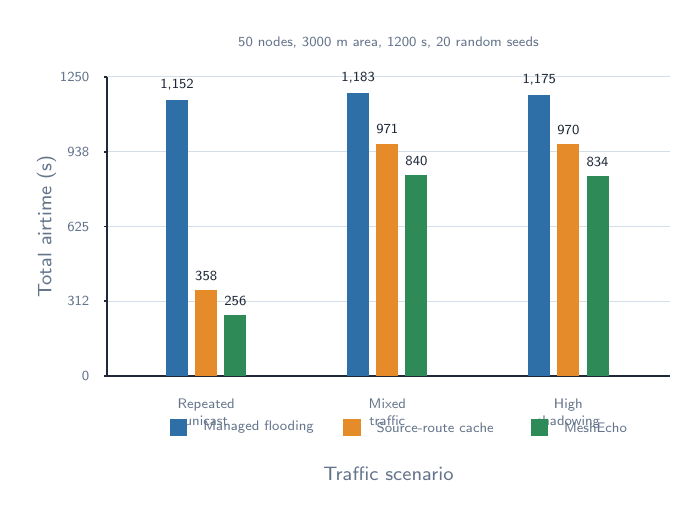
\begin{tikzpicture}[
    font=\sffamily\scriptsize,
    axis/.style={draw=ink, line width=0.65pt},
    gridline/.style={draw=grid, line width=0.35pt},
    value/.style={font=\sffamily\tiny, text=ink, anchor=south},
    tick/.style={font=\sffamily\tiny, text=muted}
]
\def\H{3.80}
\def\W{7.15}
\foreach \y/\lab in {0/0,0.95/312,1.90/625,2.85/938,3.80/1250} {
    \draw[gridline] (0,\y) -- (\W,\y);
    \draw[axis] (0,\y) -- ++(-0.04,0);
    \node[tick, anchor=east] at (-0.10,\y) {\lab};
}
\draw[axis] (0,0) -- (0,\H);
\draw[axis] (0,0) -- (\W,0);
\node[font=\sffamily\scriptsize, text=muted, rotate=90, anchor=south] at (-0.52,\H/2) {Total airtime (s)};

% Repeated unicast: flooding, source-route cache, MeshEcho.
\fill[blue] (0.75,0) rectangle (1.03,3.502);
\fill[orange] (1.12,0) rectangle (1.40,1.089);
\fill[green] (1.49,0) rectangle (1.77,0.779);
\node[value] at (0.89,3.502) {1,152};
\node[value] at (1.26,1.089) {358};
\node[value] at (1.63,0.779) {256};

% Mixed traffic.
\fill[blue] (3.05,0) rectangle (3.33,3.598);
\fill[orange] (3.42,0) rectangle (3.70,2.953);
\fill[green] (3.79,0) rectangle (4.07,2.553);
\node[value] at (3.19,3.598) {1,183};
\node[value] at (3.56,2.953) {971};
\node[value] at (3.93,2.553) {840};

% High shadowing.
\fill[blue] (5.35,0) rectangle (5.63,3.572);
\fill[orange] (5.72,0) rectangle (6.00,2.948);
\fill[green] (6.09,0) rectangle (6.37,2.536);
\node[value] at (5.49,3.572) {1,175};
\node[value] at (5.86,2.948) {970};
\node[value] at (6.23,2.536) {834};

\node[tick, anchor=north, align=center] at (1.26,-0.17) {Repeated\\unicast};
\node[tick, anchor=north, align=center] at (3.56,-0.17) {Mixed\\traffic};
\node[tick, anchor=north, align=center] at (5.86,-0.17) {High\\shadowing};

\fill[blue] (0.80,-0.76) rectangle (1.02,-0.54);
\node[tick, anchor=west] at (1.10,-0.65) {Managed flooding};
\fill[orange] (3.00,-0.76) rectangle (3.22,-0.54);
\node[tick, anchor=west] at (3.30,-0.65) {Source-route cache};
\fill[green] (5.38,-0.76) rectangle (5.60,-0.54);
\node[tick, anchor=west] at (5.68,-0.65) {MeshEcho};

\node[font=\sffamily\scriptsize, text=muted, anchor=north] at (\W/2,-1.03)
    {Traffic scenario};
\node[font=\sffamily\tiny, text=muted, anchor=south] at (\W/2,\H+0.24)
    {50 nodes, 3000 m area, 1200 s, 20 random seeds};
\end{tikzpicture}
\end{document}
